\chapter{Installation}
\label{section:installation}
Dieses Kapitel beschreibt Schritte zur Installation von \lectStudio{}. Bevor Sie mit der Installation fortfahren, stellen Sie sicher, dass Ihr System die aufgeführten Anforderungen erfüllt.

\section{Systemanforderungen}
Stellen Sie vor der Installation sicher, dass Ihr Computer die folgenden Systemanforderungen erfüllt oder übertrifft.

\vspace{1em}
\begin{tabularx}{\textwidth}{l|l}
	\textbf{RAM} & 4 GB \\ \hline
	\textbf{Speicherplatz} & 300 MB verfügbarer Festplattenspeicher \\ \hline
	\textbf{Betriebssystem} & Linux, macOS, Windows 7 oder höher
\end{tabularx}
\vspace{1em}

\begin{info}
	Für die Aufzeichnung von Vorlesungen sind zusätzlich mindestens 400 MB erforderlich.
\end{info}

\section{lectureStudio unter Windows installieren}
\begin{enumerate}
	\item Laden Sie die neueste Version des \lectStudio{} MSI-Installations-programms von der Webseite \href{https://www.lecturestudio.org/download}{lecturestudio.org/download} herunter.
	\item Navigieren Sie zu dem Ordner, in den das MSI-Installationsprogramm heruntergeladen wurde, und klicken Sie doppelt auf dieses, um den Installationsvorgang zu starten.
	\item Windows zeigt möglicherweise den folgenden Dialog an. In diesem Fall klicken Sie auf \textbf{Weitere Informationen} und fahren Sie mit der Schaltfläche \textbf{Trotzdem ausführen} fort.

	\begin{minipage}{0.46\textwidth}
		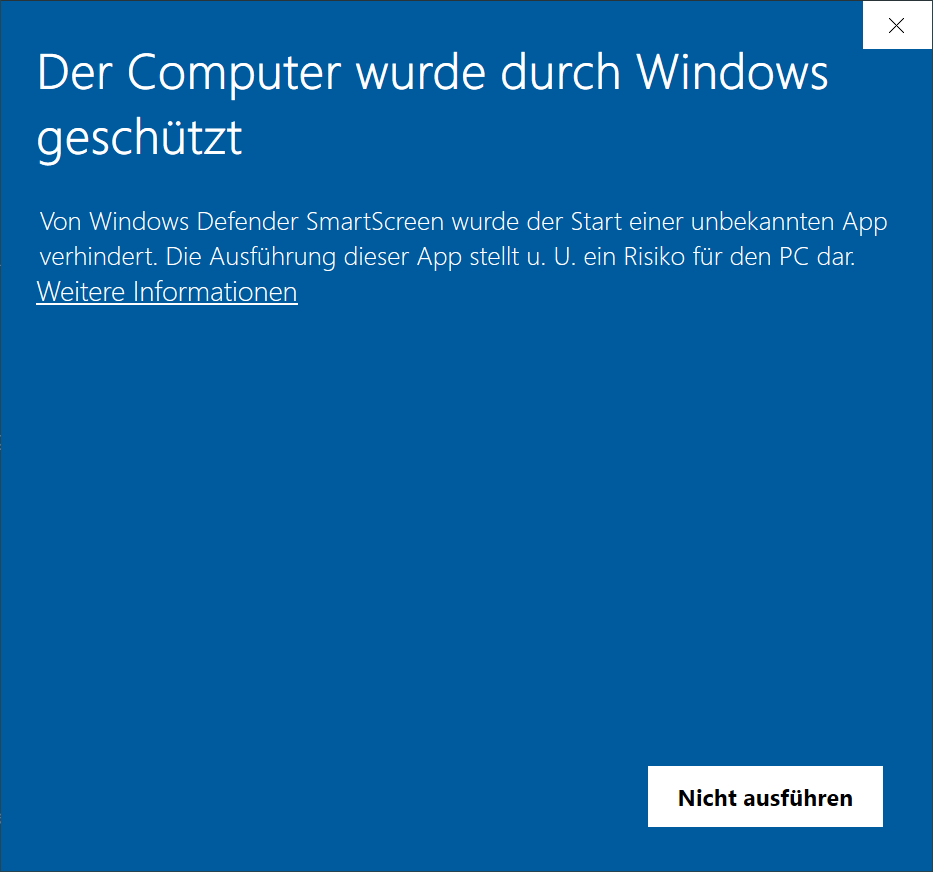
\includegraphics[width=7cm]{installation/step_1_de}
	\end{minipage}
	\begin{minipage}{0.46\textwidth}
		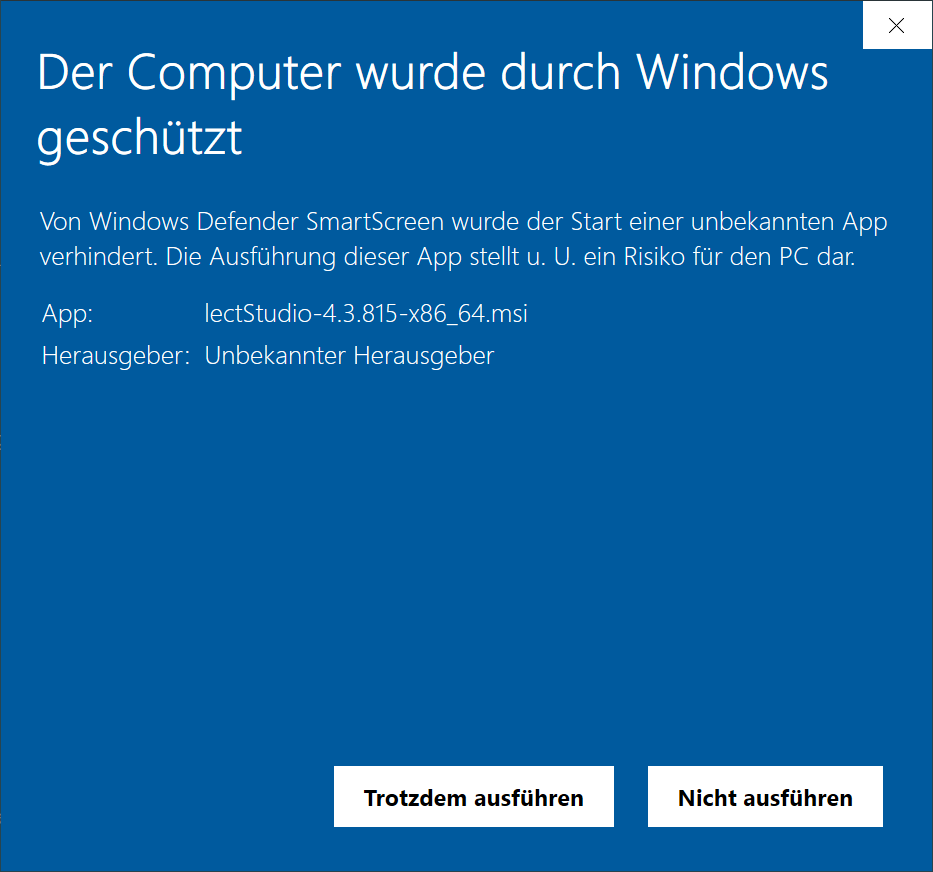
\includegraphics[width=7cm]{installation/step_1.1_de}
	\end{minipage}
	\item Nachdem das Installationsprogramm gestartet ist, akzeptieren Sie die Bedingungen in der Lizenzvereinbarung und klicken Sie auf \textbf{Install}. Um die Lizenzvereinbarung zu lesen, klicken Sie auf die Schaltfläche \textbf{License}.

	\begin{minipage}[t][][b]{0.46\textwidth}
		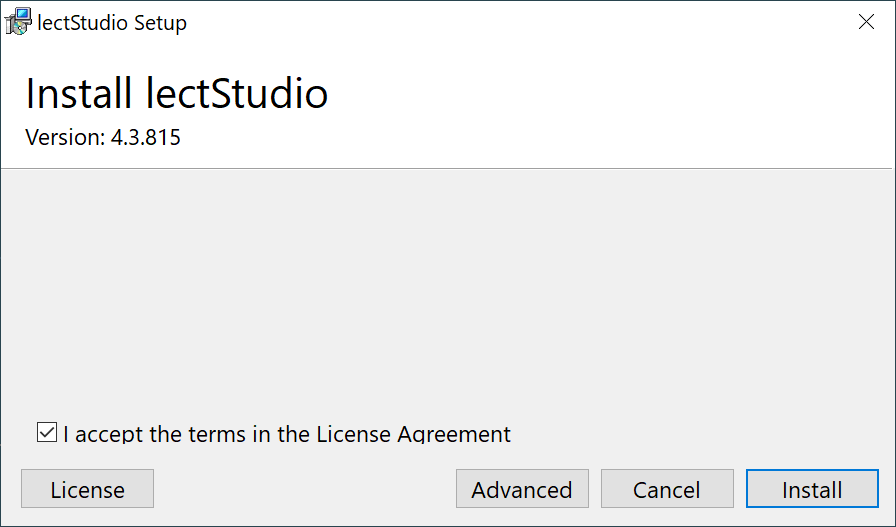
\includegraphics[width=7cm]{installation/step_2_eng}
	\end{minipage}
	\begin{minipage}[t][][b]{0.46\textwidth}
		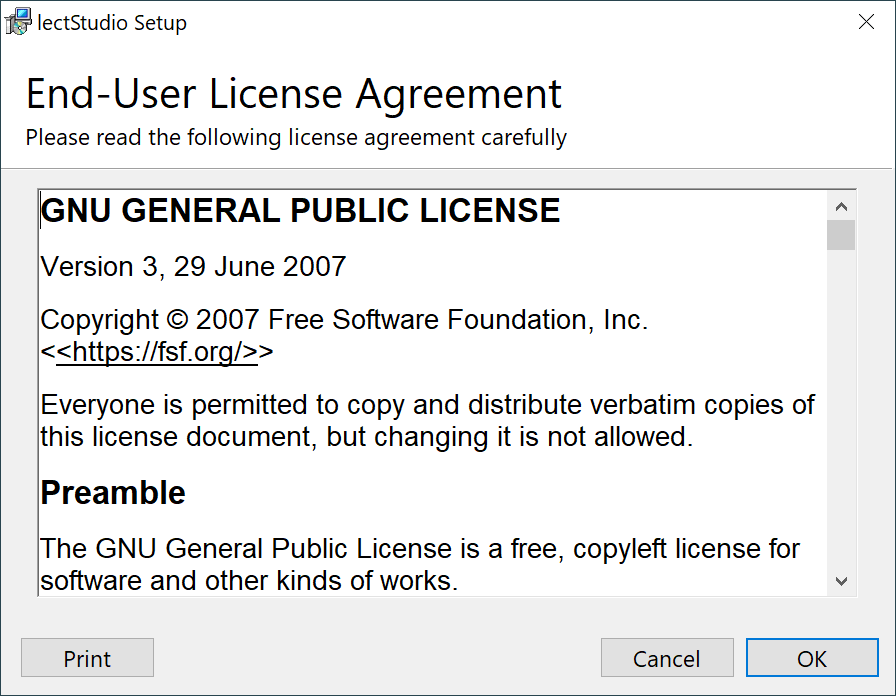
\includegraphics[width=7cm]{installation/step_2.0_eng}
	\end{minipage}

	\paragraph{Erweitertes Setup}
	Sie können die Installation von lectStudio anpassen, indem Sie auf die Schaltfläche \textbf{Advanced} klicken. Jetzt können Sie auswählen, ob auf dem Desktop und im Startmenü Verknüpfungssymbole für Anwendungen erstellt werden sollen. Um den Installationsordner zu ändern, klicken Sie auf die Schaltfläche \textbf{Change...}.

	\begin{minipage}{0.6\textwidth}
		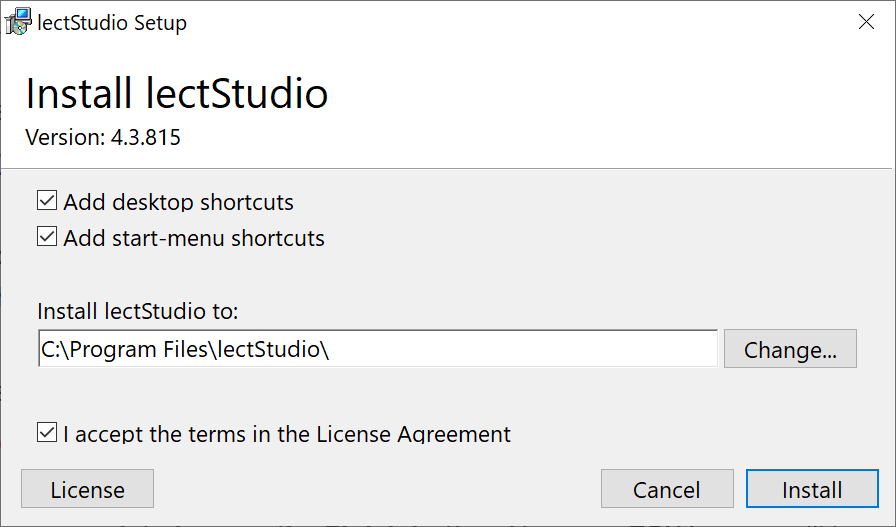
\includegraphics[width=8cm]{installation/step_2.1_eng}
	\end{minipage}

	\item Windows fordert erhöhte Berechtigungen an, damit das Installationsprogramm Änderungen an ihrem Gerät vornehmen kann. Akzeptieren Sie die Anfrage.

	\begin{minipage}{0.6\textwidth}
		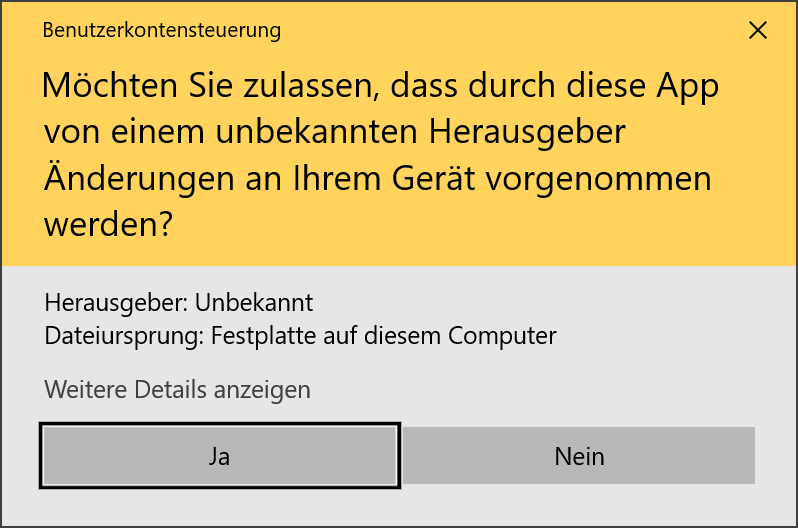
\includegraphics[width=8cm]{installation/step_3_de}
	\end{minipage}
	\item Klicken Sie auf die Schaltfläche \textbf{Finish}, wenn die Installation abgeschlossen ist.

	\begin{minipage}{0.6\textwidth}
		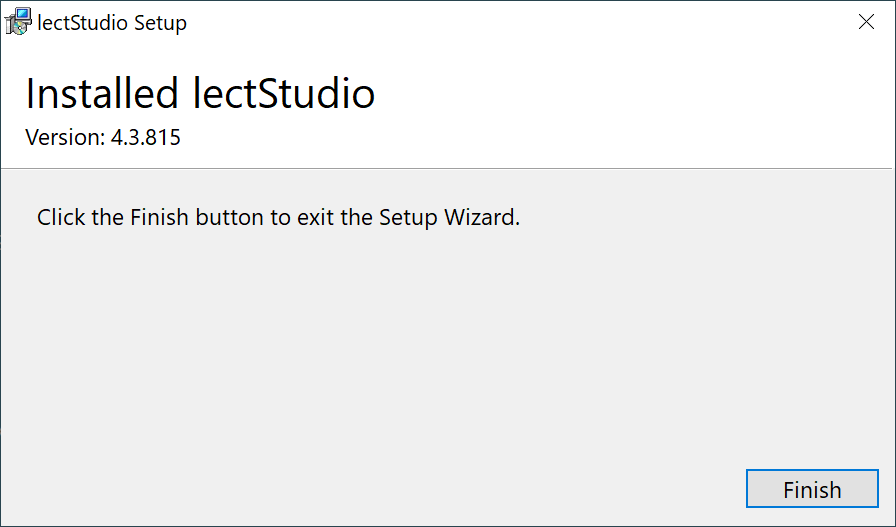
\includegraphics[width=8cm]{installation/step_4_eng}
	\end{minipage}

	\item Nach der Installation finden Sie Verknüpfungssymbole der Anwendungen auf dem Desktop und im Startmenü, wenn Sie deren Erstellung in Schritt 4 der erweiterten Einrichtung aktiviert haben.

	\begin{minipage}[t][][b]{0.4\textwidth}
		
\includegraphics[width=6cm]{installation/step_5.0_eng}
	\end{minipage}
	\begin{minipage}[t][][b]{0.4\textwidth}
		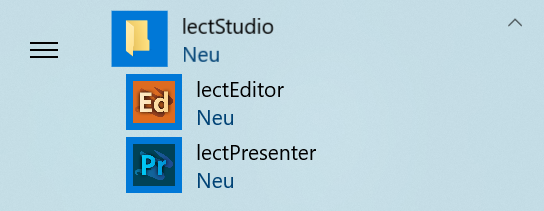
\includegraphics[width=6cm]{installation/step_5.1_de}
	\end{minipage}
 \end{enumerate}


 \section{lectureStudio unter Linux installieren}
 \begin{enumerate}
	\item Laden Sie das Archiv der neuesten \lectStudio{}-Version von der Webseite \href{https://www.lecturestudio.org/download}{lecturestudio.org/download} herunter.
	\item Navigieren Sie zu dem Ordner, in den das Archiv heruntergeladen wurde.
	\item Entpacken Sie die Datei mit dem Namen \lectStudio{}-x.y.z-linux-x86\_64.zip (wobei x.y.z die Versionsnummer ist).
	\\\\
	Sie können das Archiv über das Kontextmenü der grafischen Bedienoberfläche oder über die Kommandozeile entpacken.
	\\\\
	\textbf{In der Kommandozeile entpacken:}
	\begin{command}
		unzip \lectStudio{}-x.y.z-linux-x86\_64.zip
	\end{command}
	\item Kopieren Sie das entpackte \lectStudio{}-Verzeichnis an sein endgültiges Ziel.
	\item Die Anwendungen sind im Verzeichnis \inlinecode{bin} des \lectStudio{} Verzeichnisses zu finden.
\end{enumerate}

 \section{lectureStudio unter macOS installieren}
 \begin{enumerate}
	\item Laden Sie die neueste Version des \lectStudio{} PKG-Installations-programms von der Webseite \href{https://www.lecturestudio.org/download}{lecturestudio.org/download} herunter.
	\item Navigieren Sie zu dem Ordner, in den das PKG-Installationsprogramm heruntergeladen wurde, und klicken Sie doppelt auf dieses, um den Installationsvorgang zu starten.
	\item Nachdem das Installationsprogramm gestartet ist, fahren Sie nach der Einführung fort und akzeptieren die Bedingungen in der Lizenzvereinbarung. Um die Lizenzvereinbarung zu lesen, klicken Sie auf die Schaltfläche \textbf{Lizenz lesen}. Nachdem Sie die Lizenzvereinbarung akzeptiert haben, klicken Sie auf \textbf{Fortfahren}.

	\begin{minipage}[t][][b]{0.46\textwidth}
		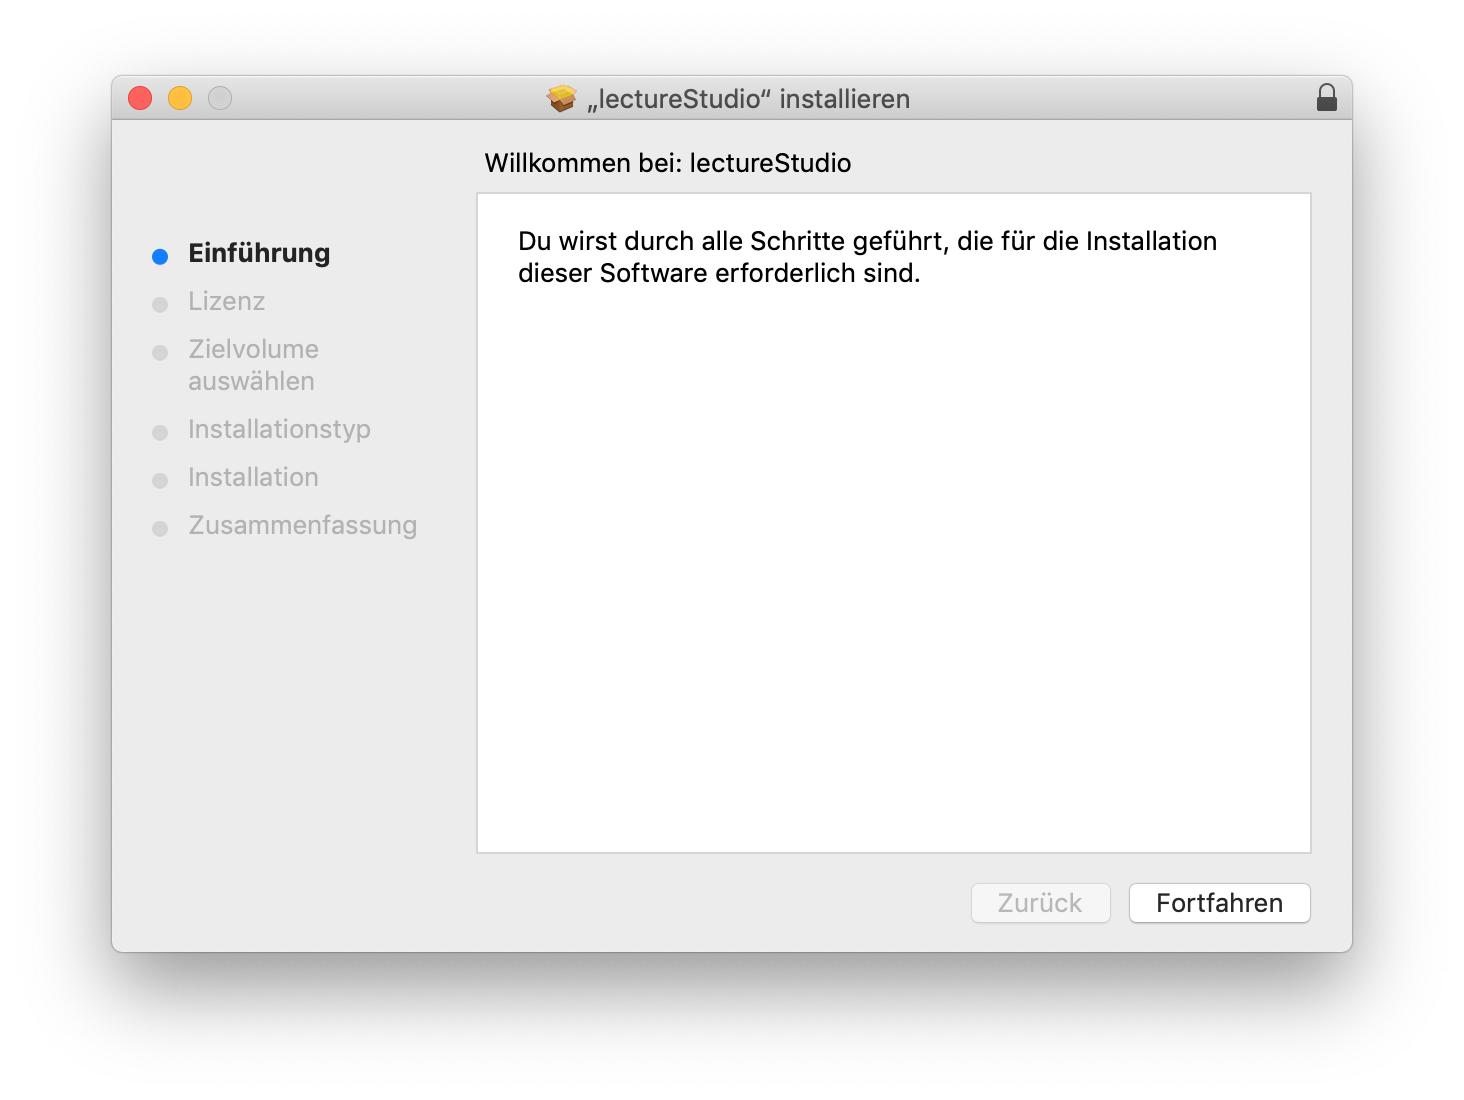
\includegraphics[width=7cm]{installation/mac-install-1}
	\end{minipage}
	\begin{minipage}[t][][b]{0.46\textwidth}
		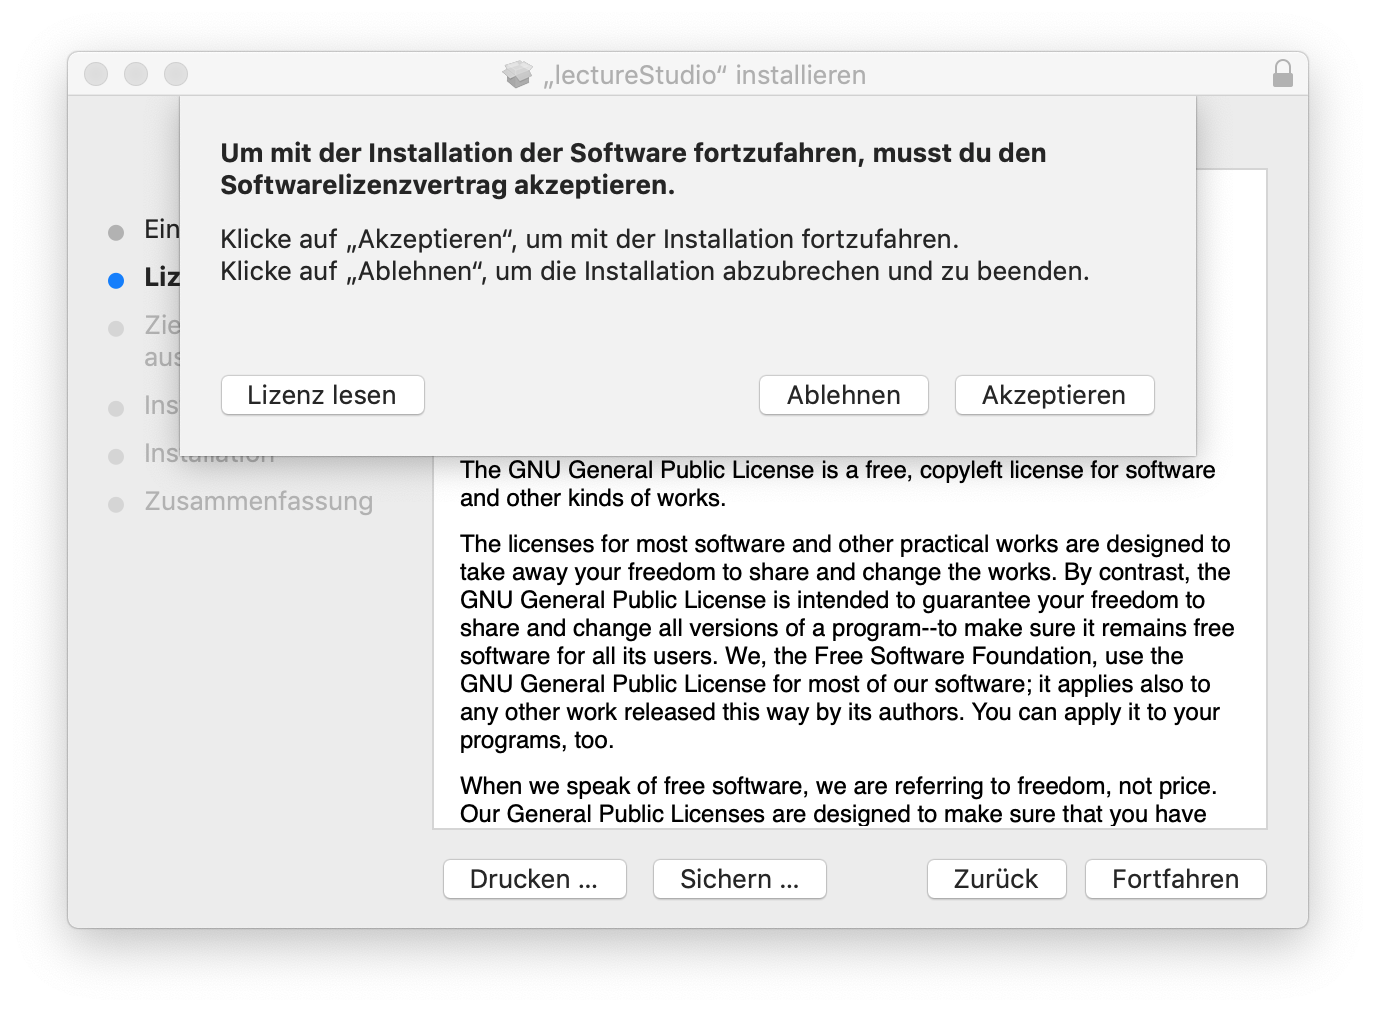
\includegraphics[width=7cm]{installation/mac-install-2}
	\end{minipage}

	\item Nun können Sie \lectStudio{} auf dem Laufwerk installieren. Klicken Sie auf \textbf{Installieren}. macOS fordert erhöhte Berechtigungen an, damit das Installationsprogramm Änderungen an ihrem Gerät vornehmen kann. Geben Sie hierfür Ihren Benutzernamen und das dazugehörige Passwort ein und klicken auf \textbf{Software installieren}.
	
	\begin{minipage}[t][][b]{0.46\textwidth}
		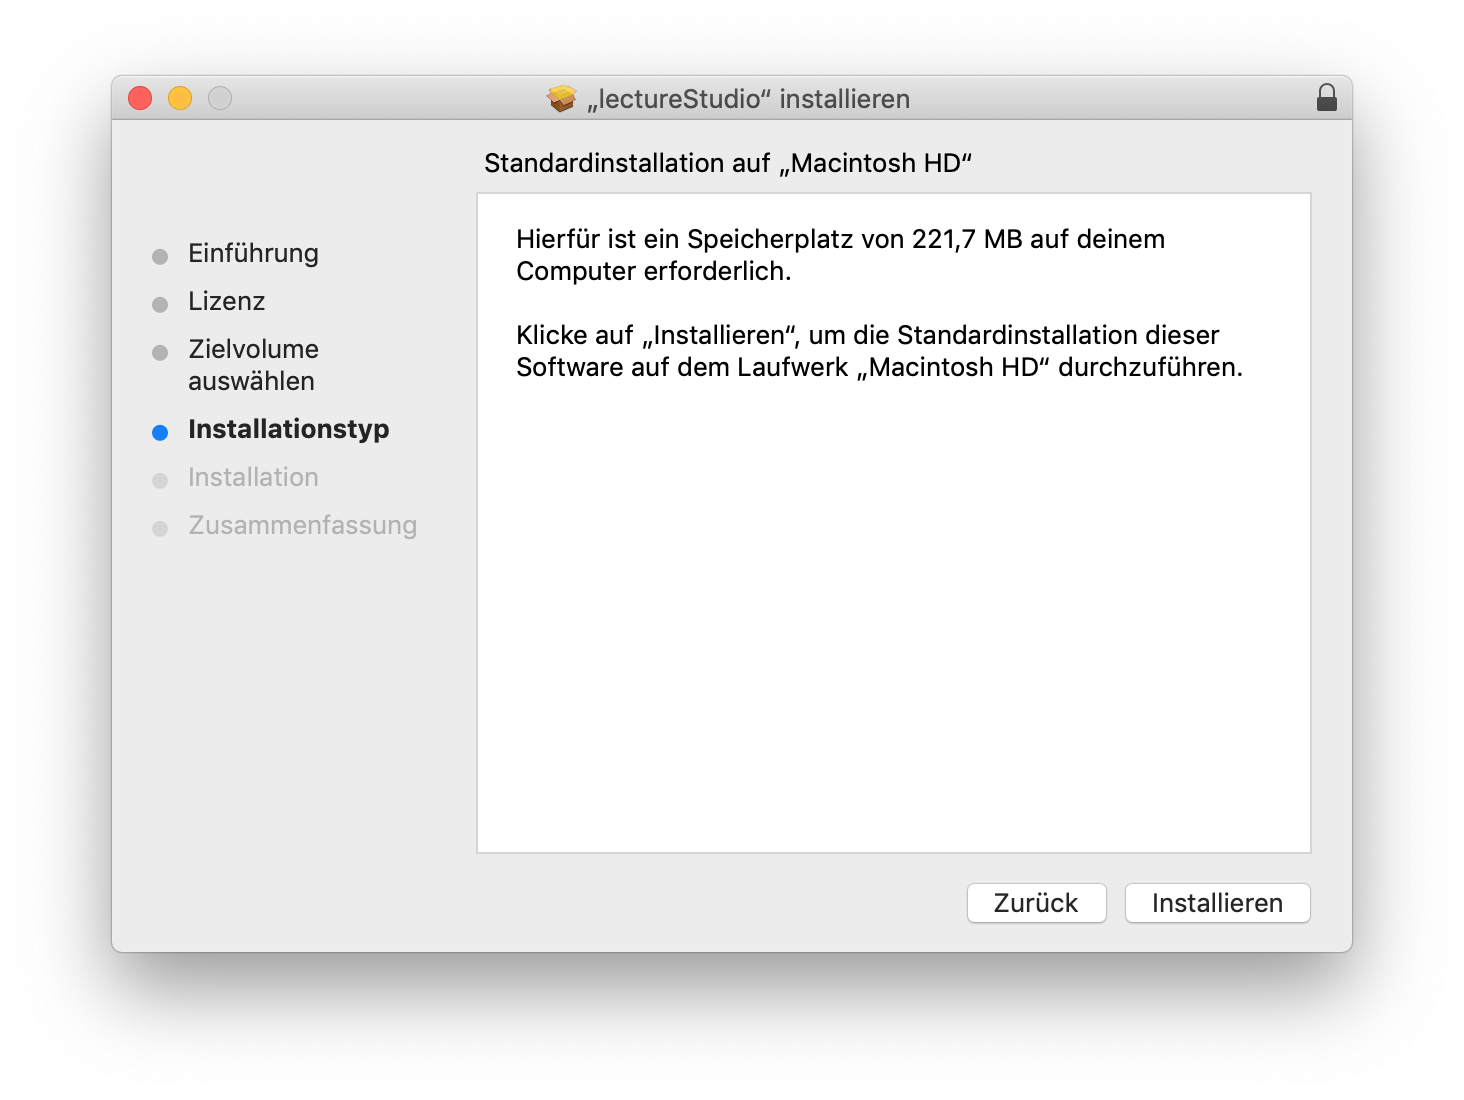
\includegraphics[width=7cm]{installation/mac-install-3}
	\end{minipage}
	\begin{minipage}[t][][b]{0.46\textwidth}
		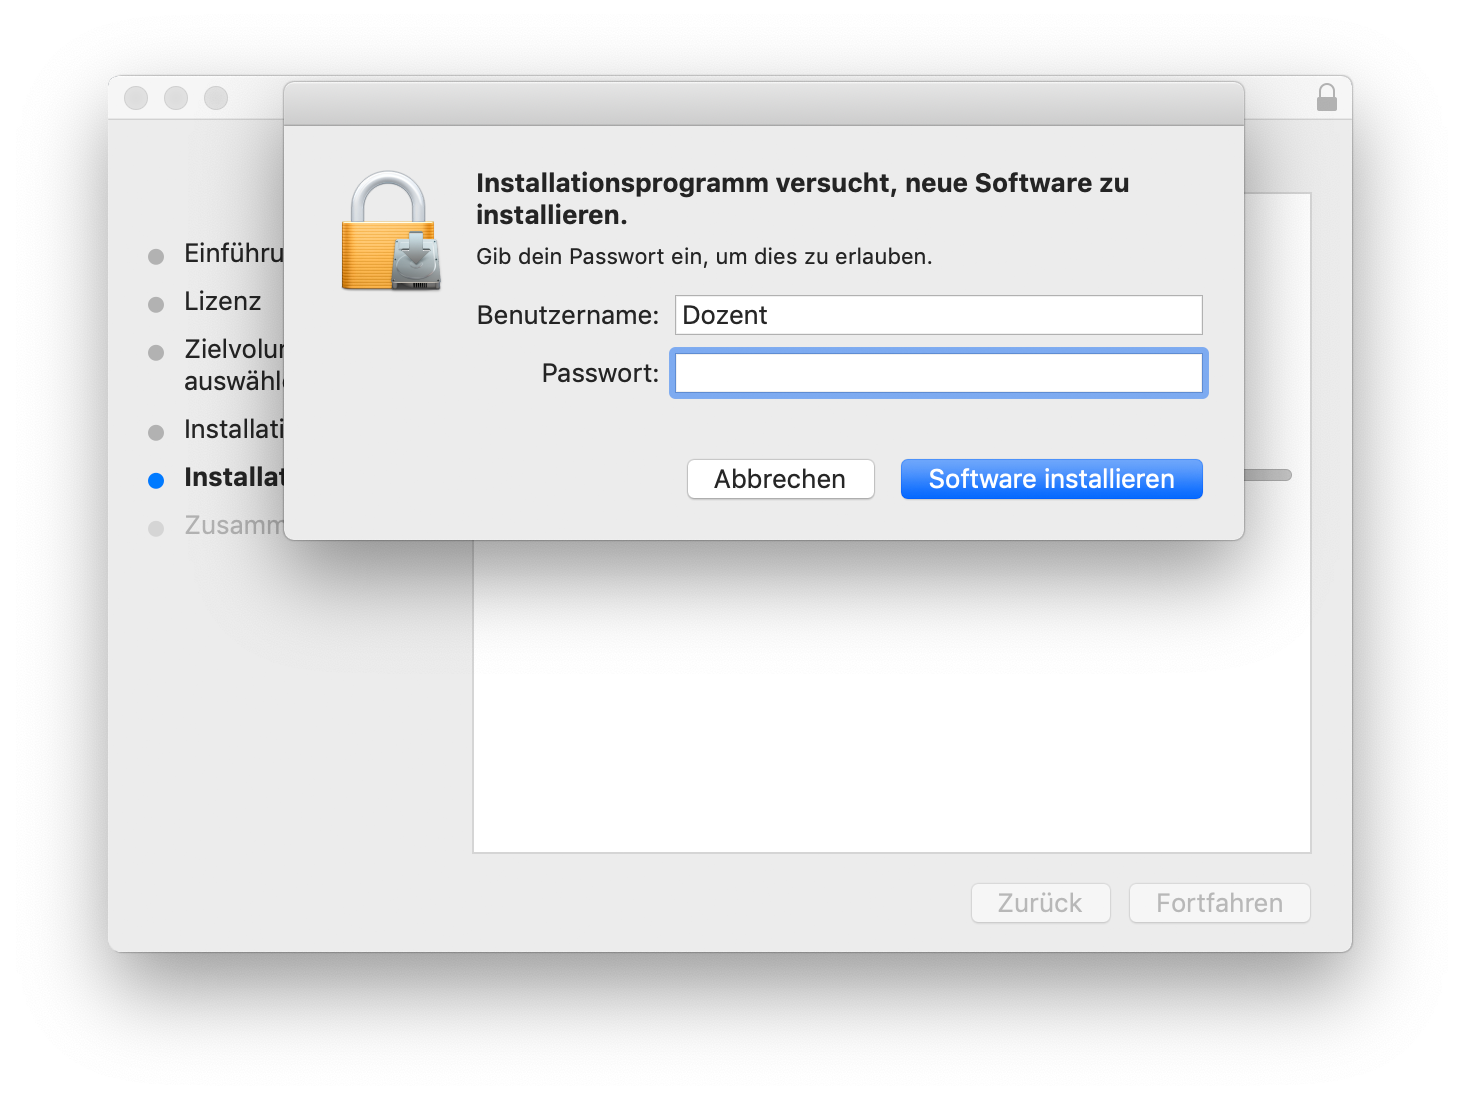
\includegraphics[width=7cm]{installation/mac-install-4}
	\end{minipage}

	\item Sobald die Installation erfolgreich abgeschlossen ist, klicken Sie auf die Schaltfläche \textbf{Schließen}.

	\begin{minipage}{0.6\textwidth}
		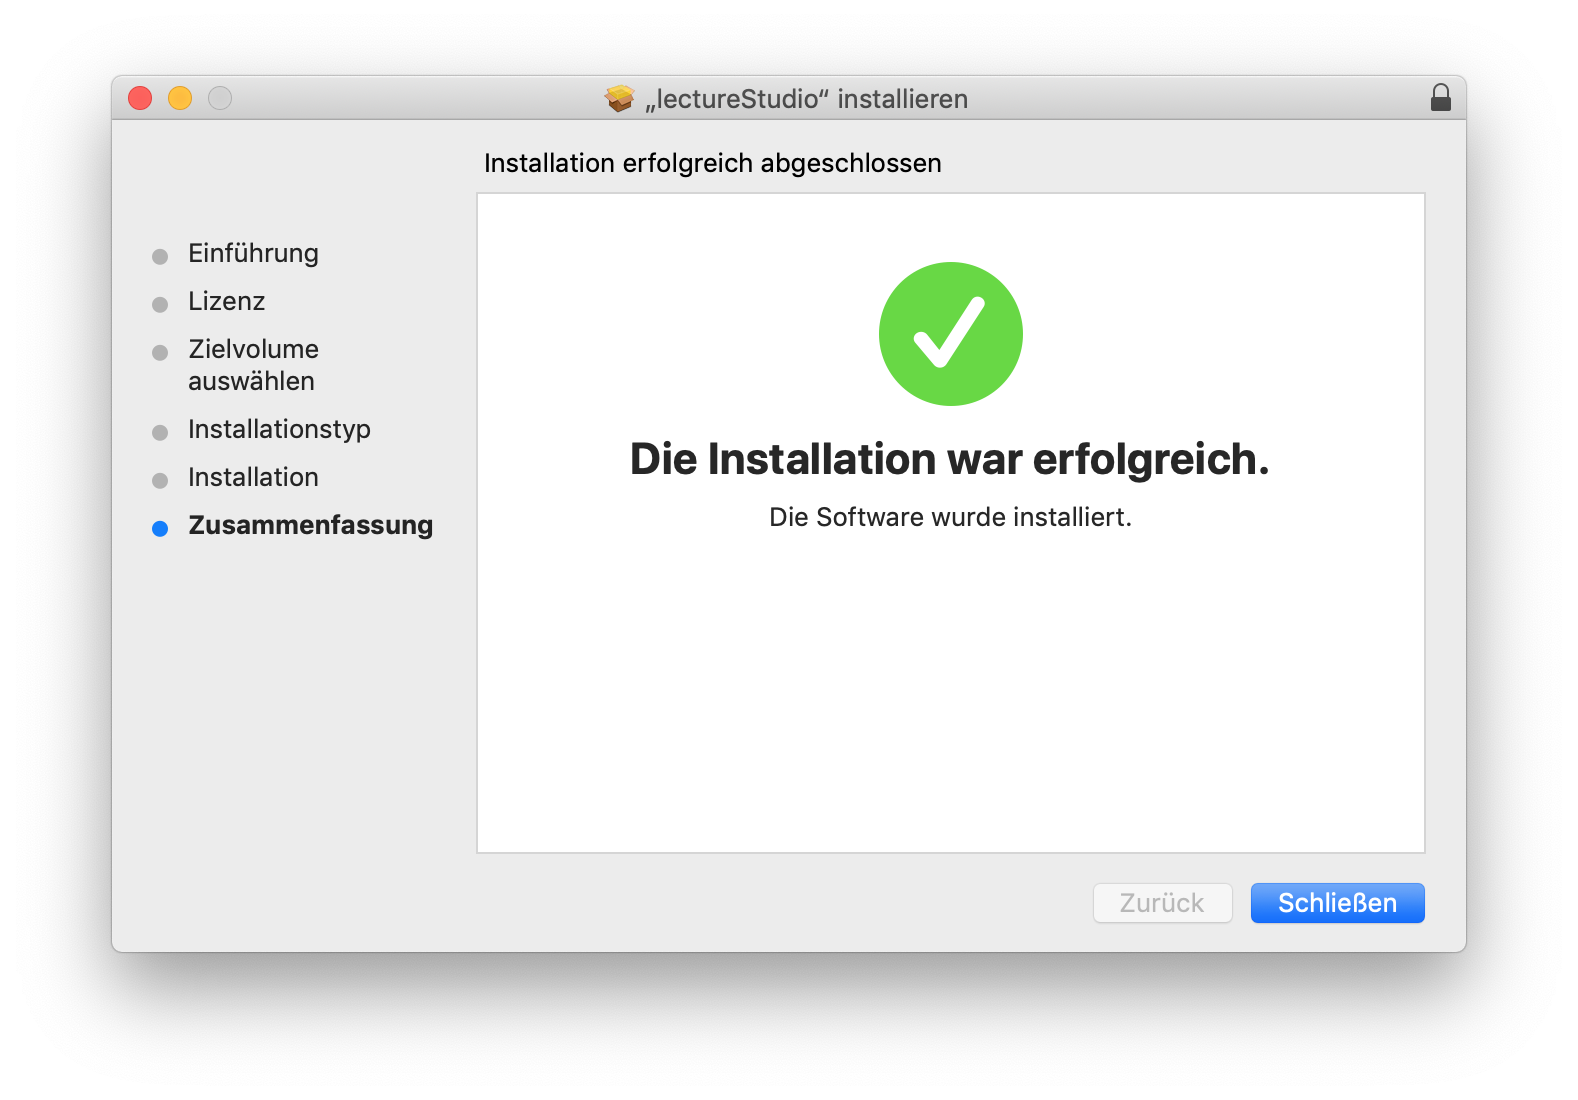
\includegraphics[width=7cm]{installation/mac-install-5}
	\end{minipage}

	\item Nach der Installation finden Sie die installierten Anwendungen im Launchpad.

	\begin{minipage}[t][][b]{0.46\textwidth}
		
\includegraphics[width=5cm]{installation/mac-install-6}
	\end{minipage}
\end{enumerate}